\section{Classical conditional linear references}\label{app:linear}
\begin{proposition}[Fourier features are a GP prior; Bochner]\label{prop:bochner}
Let $f(u)=\sum_{j=1}^m w_j\varphi_j(u)$ with
$\varphi_j(u)=\sqrt{2/m}\cos(2\pi b_j^\top u+c_j)$, $b_j\sim p(b)$,
$c_j\sim\mathcal{U}[0,2\pi)$ and $w\sim\mathcal{N}(0,s^2I)$. As
$m\to\infty$, $f$ is a zero-mean stationary Gaussian process with covariance
$k(h)=s^2\,\mathbb{E}_b[\cos(2\pi b^\top h)]$ and spectral density
$S(\nu)=s^2[p(\nu)+p(-\nu)]/2$, equal to $s^2p(\nu)$ for symmetric $p$.
\end{proposition}
Hence a ridge read-out of Fourier features is the GP posterior mean under
prior spectrum $S$; with $p=\mathcal{N}(0,\sigma^2I)$,
$S(\nu)\propto\exp(-\|\nu\|^2/2\sigma^2)$. Tuning $\sigma$ (SuperF) or
choosing frequency parameters from a target spectrum (FreSh, WINNER, SEC)
controls frequency preference; the exact GP interpretation applies to the linear feature readout within a restricted family; a GP with a fitted or
known spectrum picks it directly. For an MLP on Fourier features trained by
gradient descent, the lazy-training limit gives kernel regression with a
stationary NTK modulated by $p$ \citep{tancik2020fourier,jacot2018ntk}, under additional architectural and optimisation assumptions. General trained MLPs and grid fields do not thereby have known stationary spectral priors; we compare their behaviour empirically
(\S\ref{sec:exp-ab}).

\begin{proposition}[Covariance-conditioned linear optimality]\label{prop:bound}
For zero-mean or correctly centred signal and noise, let $x$ have covariance $C_P$, uncorrelated noise covariance $\sigma_n^2I$, and positive-definite $C_y$. Every linear
estimator $\hat x=Gy$ satisfies
$\mathbb{E}\|x-\hat x\|^2\ge\mathbb{E}\|x-\hat x_{\mathrm{LMMSE}}(P)\|^2$,
with $\hat x_{\mathrm{LMMSE}}(P)=C_PA^\top(AC_PA^\top+\sigma_n^2I)^{-1}y$.
\end{proposition}
This optimum holds in expectation under the specified covariance and noise.
Second moments and zero signal--noise cross-covariance suffice for linear
optimality; joint Gaussianity additionally identifies the conditional mean
with MMSE. A generic spectrum does not define a distribution-free ceiling
on real images, and an image periodogram is an oracle reference rather than
an attained optimality certificate. For any fixed linear $H$ and evaluation
map $W$, with $C_y=AC_PA^\top+C_n$ positive definite,
\begin{align*}
&\mathbb E\|W(x-Hy)\|^2-\mathbb E\|W(x-H_Py)\|^2\\
&=\operatorname{tr}[W(H-H_P)C_y(H-H_P)^\top W^\top]\ge0,
\end{align*}
where $H_P=C_PA^\top C_y^{-1}$. The same covariance-conditioned optimum
minimises total and projected linear risk.

\paragraph{Closed form for decimation.} For ideal periodic $A$ = blur $K$ followed by
decimation by $s$, each LR frequency $\omega$ collects $s^d$ HR frequencies
$\nu_m=\omega+m/s$, and
\begin{equation}\label{eq:alias}
R(\nu_0)=\frac{|\hat K(\nu_0)|^2P(\nu_0)}{\sum_m|\hat K(\nu_m)|^2P(\nu_m)+N_\omega}.
\end{equation}
The sum in the denominator is aliasing. The historical simulations show little change over the particular tested noise range (Table~\ref{tab:map}); this is not a general noise-insensitivity claim.

Here $N_\omega$ is noise power under a compatible Fourier normalisation.
Changing other powers within the alias set changes the effective noise;
the scalar mismatch identity assumes that effective noise is fixed.
Finite crops, boundary interpolation, rotations and sparse sampling
normally require the matrix risk expression above. F1/G1 use HR256 and 73 images;
L1/L2 use HR240 and 74, with their own window and pooling conventions.
Empirical recovery can be negative and need not equal reference recovery.

Zero-noise singular cases require a pseudoinverse or explicitly stated
regularisation. A numerical noise floor changes the estimator; its value
must not replace the physical observation-noise covariance in risk evaluation.


\section{Classical mismatch costs and diagnostic limits}\label{app:mismatch}
For a centred scalar observation with fixed effective noise variance $q$ and signal variance $p$, the matched Wiener gain is $R=p/(p+q)$. An estimator assuming variance $\kappa p$ uses $g=\kappa R/(1-R+\kappa R)$. The normalised excess error is a classical identity:
\begin{proposition}[Scalar mismatch cost]\label{prop:mismatch}
\begin{equation}\label{eq:delta}
\Delta(R,\kappa)=\frac{R(1-R)^2(\kappa-1)^2}{(1-R+\kappa R)^2}.
\end{equation}
\end{proposition}
The proof in Appendix~\ref{app:proof} separates this identity from its experimental approximations. In absolute units, for true power $P$, assumed power $Q$ and unchanged effective noise $N$,
\begin{equation}\label{eq:delta-abs}
P\Delta=\frac{N^2(Q-P)^2}{(P+N)(Q+N)^2}.
\end{equation}
Under-estimation has limit $\Delta\to R$ as $\kappa\to0$, whereas over-estimation has limit $(1-R)^2/R$ as $\kappa\to\infty$. The latter exceeds signal energy at $R<(3-\sqrt5)/2$; total error exceeds zero reconstruction when $\Delta>R$. Neither statement defines a universal safe bandwidth.
\begin{corollary}[Reciprocal mismatch]\label{cor:flip}
For $0<R<1$ and $\kappa>1$, $\Delta(R,\kappa)>\Delta(R,1/\kappa)$ if and only if $R<1/2$.
\end{corollary}
The effective noise is held fixed, including any aliased components represented by it. Changing several powers in an alias set or using a non-diagonal sampling operator need not preserve this scalar reduction.

\begin{figure*}[t]\centering
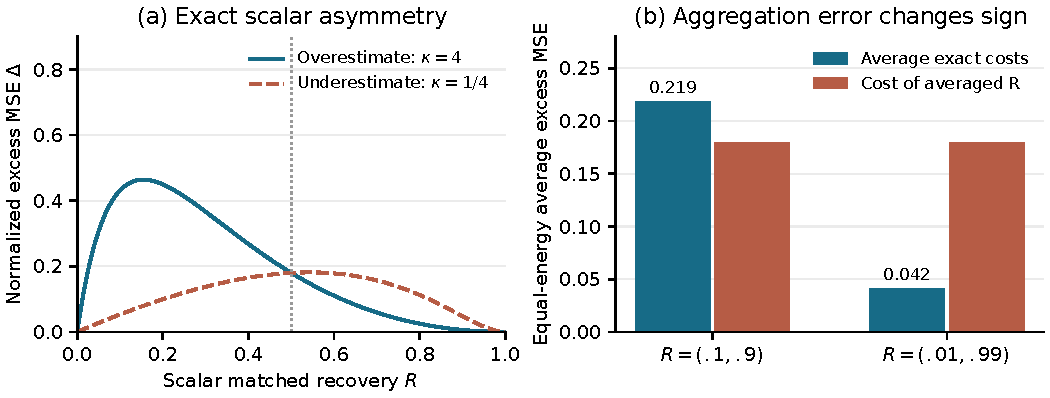
\includegraphics[width=.95\textwidth]{figures/scalar-cost.pdf}
\caption{Classical scalar cost and aggregation limits. Reciprocal mismatches cross at $R=.5$ under fixed effective noise. Equal-energy modes with the same mean $R=.5$ and $\kappa=4$ can give aggregation errors of either sign. These calculations do not identify a nonlinear network's effective prior.}\label{fig:cost}
\end{figure*}

\paragraph{Reference labels, not natural boundaries.} Historical protocols partition reference recovery at $.1$ and $.8$: A denotes high reference recovery, B intermediate and C low. These fixed labels permit the original test criteria to be audited. Their sensitivity has not been established, so we do not recommend them as deployment thresholds. With a fixed finite $\kappa$, the scalar excess vanishes as $R\to0$ or $1$, but the low-$R$ limit is not uniform over large mismatch factors. No reference label identifies the causal bottleneck of a trained decoder.

\paragraph{Band approximation.} A diagnostic sum
\begin{equation}\label{eq:crit}
C(Q)=\sum_b E_b\,\Delta\big(R_b,\kappa_b(Q)\big)
\end{equation}
substitutes measured band energies, reference recoveries and ratios of spectrum integrals. It is not the exact risk for a general operator. Its ranking accuracy and winner selection are distinct tests (\S\ref{sec:boundary}). Averaging $R$ and $\kappa$ before the nonlinear formula can either over- or under-estimate the true sum. For a fixed linear estimator the matrix expression in Appendix~\ref{app:linear} instead evaluates the specified covariance law directly.

\paragraph{No network mechanism follows.} A trained ASISR decoder is not a fixed Wiener estimator with known $\kappa$. Its measured $\Rnet$ is a truth-dependent outcome. Values near zero or one do not force a small readout-ablation loss: removing a component may improve a poorly recovered band or damage a perfectly recovered one. The loss ordering and scale-marginalisation tests in the main text therefore require empirical evidence independent of the scalar identity.

\section{Proof of Proposition~\ref{prop:mismatch}}\label{app:proof}
With $R=p/(p+q)$ the matched gain $R$ attains error $p(1-R)$. The gain
$g=\kappa p/(\kappa p+q)=\kappa R/(\kappa R+1-R)$ gives error
$(1-g)^2p+g^2q$. Using $q/p=(1-R)/R$ and $D=\kappa R+1-R$,
\[
\frac{(1-g)^2p+g^2q}{p}=\frac{(1-R)\big[(1-R)+\kappa^2R\big]}{D^2}.
\]
Subtracting $(1-R)$ and expanding $D^2$, the numerator becomes
$(1-R)\,R(1-R)(\kappa-1)^2$, which is Eq.~\eqref{eq:delta}.
For Cor.~\ref{cor:flip},
$\Delta(R,\kappa)/\Delta(R,1/\kappa)=\big((1-R)\kappa+R\big)^2/\big(1-R+\kappa R\big)^2$,
which exceeds 1 for $\kappa>1$ iff $(\kappa-1)(1-2R)>0$, i.e.\ iff $R<1/2$
(also checked numerically).

\section{Reproducibility}
Original sources, protocols and results retain their server directory
names in the collected evidence. The updated \texttt{SOURCES.md} maps each
claim to original or new output. New G1 and L2 runs invoke original frozen
evaluation code and preserve old results. The G1 protocol matches SHA256
prefix \texttt{548b26fe}; the full hash is recorded in \texttt{SOURCES.md}.
Independent L2 checking reconstructs pooled recoverability from saved
per-image signal/error arrays; G1 checking validates saved pooled numbers
and coverage, but per-image energy weights were not saved by its original
script. Exact machine-readable numerical checks accompany the evidence.

\section{Historical reference map}\label{app:map}
These prior simulations retain the original numerical values and fixed labels for source traceability. They do not use the natural-image E3 observation law: the latter has no injected noise and uses a different numerical variance. The labels are descriptive, with threshold sensitivity unverified.
\begin{table*}[t]\centering\small
\caption{Historical reference simulations: $\Rlin$ per band under the generic
$1/f^2$ prior, assumed spectrum and simulated observations; not a natural-image bound \src{OUT3/d8}.
Labels: A $\ge0.8$, B, C $<0.1$.}\label{tab:map}
\begin{adjustbox}{max width=\linewidth}\begin{tabular}{llccc}\toprule
Task & $\sigma_n$ & $b_1$ & $b_2$ & $b_3$\\\midrule
Single image $\times2$ & .002 / .01 & 1.00 / 1.00 & .92 / .90 & .09 / .08\\
Single image $\times4$ & .002 / .01 & .98 / .98 & .09 / .08 & .01 / .01\\
Single image $\times8$ & .002 / .01 & .79 / .77 & .01 / .01 & .01 / .01\\
Sparse 5\% & .002 & .70 & .09 & .03\\
Sparse 10\% & .002 & .81 & .20 & .07\\
Sparse 25\% & .002 & .92 & .47 & .20\\
Sparse 50\% & .002 & .98 & .76 & .46\\
Multi-frame $\times4$, $T{=}4$ & .002$\to$.02 & $\approx$1.0 & .73$\to$.51 & .12$\to$.03\\
Multi-frame $\times4$, $T{=}8$ & .002$\to$.02 & $\approx$1.0 & .83$\to$.62 & .27$\to$.08\\
Multi-frame $\times4$, $T{=}16$ & .002$\to$.02 & $\approx$1.0 & .90$\to$.73 & .41$\to$.15\\
\bottomrule\end{tabular}\end{adjustbox}
\end{table*}


\section{Matrix optimality and aggregation counterexamples}
Let $e_P=x-H_Py$. Since $\mathbb E[e_Py^\top]=0$, expanding
$x-Hy=e_P+(H_P-H)y$ cancels both cross terms. Multiplication by an arbitrary
fixed $W$ and taking traces gives the identity in Appendix~\ref{app:linear}.
Gaussianity is unnecessary for this second-moment calculation.

Even equal-energy modes with identical $\kappa=4$ demonstrate that band
plug-in costs have no uniform error direction. For $R=(.1,.9)$ the average
exact cost is .218639; for $R=(.01,.99)$ it is .041601. Both have average
$R=.5$, whose plug-in cost is .18: an underestimate in the first example
and an overestimate in the second. These examples do not use non-diagonal
sampling, so aggregation alone suffices. For fixed finite $\kappa>0$ the
cost vanishes as $R\to0$ or $1$, but the low-$R$ limit is not uniform in
$\kappa$: $R=.01$, $\kappa=100$ gives $\Delta=24.256863$.
The scalar identity was independently checked on a $101\times121$ grid
with maximum algebraic residual $7.2\times10^{-15}$ \src{CPU-10000}.


\section{Exploratory same-observation linear controls}\label{app:controls}
This development diagnostic separates a model's own uncertainty from
actual reconstruction error. It uses two already-seen images, DIV2K
0801/0802, one Fourier-feature seed and one paired noise draw; it is
neither a confirmatory comparison nor a new selection method.
A central native $128\times128$ crop is average-pooled to $64\times64$.
Two point-sampling frames use vertical stride four and horizontal phases
$(0,0)$, $(0,1)$ or $(0,2)$, each with 512 noisy RGB observations and
noise variance $\nu=10^{-4}$. Only horizontal phases change; this matched
point operator differs from E1's native integrated footprints.

All 24 linear predictions are fixed before truth-based scoring: two
images, three geometries, two scales $\sigma\in\{3,10\}$ and two kernels.
The RBF is $k_\sigma(u,v)=\exp[-2\pi^2\sigma^2\|u-v\|^2]$. The finite
Fourier kernel uses the original network's 256 frozen Gaussian frequencies,
with $\phi(u)=[\cos(2\pi Bu),\sin(2\pi Bu)]/\sqrt{256}$ and
$k(u,v)=\phi(u)^\top\phi(v)$. Both have unit diagonal, fixed mean $m=.5$
and ridge parameter $\nu$, solved in float64 by Cholesky. No bandwidth,
amplitude or regularisation search is performed. Saved nonlinear FF
outputs are compared without retraining. Fixed Fourier ridge is not the
MLP's full NTK or learned kernel \citep{tancik2020fourier}; its mean,
regularisation and optimisation also differ from those of the FF network.
The noise generator resets to the same seed for each geometry, giving
common random numbers across geometries.

Let $T=K_{to}(K_{oo}+\nu I)^{-1}$ for the $P$ scored target pixels.
Conditioning on a fixed clean RGB image, the exact raw-output risk over
fresh observation noise is
\begin{equation*}
\frac{\|T(X_o-m)-(X_t-m)\|_F^2}{3P}
+\frac{\nu\|T\|_F^2}{P}.
\end{equation*}
Truth is used only to score the bias term after the complete prediction
cohort is hash-frozen. For the saved noise draw, actual raw MSE further
includes its realised noise term and signed bias--noise cross term.
These identities do not apply after clamping, and are not observation-only
risk estimators. In contrast, $\operatorname{diag}(K_{tt}-TK_{ot})$ is
uncertainty under the candidate's own Gaussian prior. Different kernels
specify different target laws, so their own uncertainties are not a common
actual-risk comparison.

\begin{table}[t]
\centering\small
\begin{tabular}{lrrr}
\toprule
Estimator & $\sigma$ & 0801 & 0802 \\
\midrule
RBF & 3 & $+.763$ & $+.552$ \\
RBF & 10 & $+1.792$ & $+1.908$ \\
Fixed Fourier ridge & 3 & $+.480$ & $-1.125$ \\
Fixed Fourier ridge & 10 & $-.647$ & $-.664$ \\
Trained FF & 3 & $+.633$ & $+.443$ \\
Trained FF & 10 & $+.951$ & $+.919$ \\
\bottomrule
\end{tabular}
\caption{Development difference in clamped PSNR (dB), phase $(0,2)$ minus
$(0,1)$, on the identical shave-four region. All opposing signs are
retained; these two images and one seed do not establish a population
ordering or a nonlinear mechanism.}\label{tab:controls}
\end{table}

Table~\ref{tab:controls} has three opposing finite-Fourier comparisons.
At $\sigma=10$, phase $(0,2)$ has conditional expected \emph{raw} MSE
1.901/2.473 on 0801/0802, predominantly bias; clipping must not conceal
this failure. Within each fixed kernel/scale, model posterior variance
orders the three phases as $02<01<00$, while the conditional noise
propagation term orders them as $00<02<01$. Total conditional raw-risk
ordering agrees with model variance in only five of eight image/kernel/
scale combinations. Lower self-prior uncertainty therefore does not
certify lower fixed-image error.

On the discrete $56\times56$ target crop, phases $(0,1)$ and $(0,2)$
have exactly the same nearest-observation distance histogram. Continuous
periodic maximum gaps three/two alone cannot explain their different
errors, especially for these nonperiodic kernels and nonnested observation
sets. Covariance-parameter identifiability and reconstruction error are
different objects; this diagnostic supplies no general transfer theorem.
Joint correlations, prior mismatch and estimator behaviour require
separate analysis rather than a nearest-distance or rank-only mechanism.

All 24 controls finish with no numerical failure in 17.39 seconds of
shared CPU wall time (four threads, nice 10, 600-second absolute budget).
The complete prediction manifest precedes scoring; all saved outputs,
linear responses, residuals and failures are retained. Independent LU
recomputation of all 24 controls and primal/dual checking of all 12
Fourier controls agree with predictions within $2.51\times10^{-11}$.
These audits validate the calculations, not natural-image prior validity,
practical guidance or publication novelty \src{CTRL-20261008}.

As a common-law diagnostic, the same 12 distinct saved linear responses
are evaluated on 32 separate calibration crops, DIV2K 0001--0032, with
identical preprocessing, mean, noise variance and target region. Averaging
the preceding conditional-risk formula over these complete RGB images
defines a finite empirical evaluation law; no Gaussian or stationarity
assumption or population confidence interval is attached to it. All 384
image/operator risks and eight static recommendations are hash-frozen
before consulting the two development images. This is a retrospective
diagnostic designed after their earlier outcomes, not prospective evidence.
Calibration chooses RBF $\sigma=3$ within every geometry, and phase $(0,2)$
globally, agreeing with the conditional-risk optimum on both development
images. Across the overlapping eight choice groups per image, 15 of 16
recommendations match their oracle; the exception is Fourier ridge
$\sigma=3$ on 0801, with raw-risk regret .001037. Nevertheless, 15 of 132
pairwise comparisons have opposing signs. These dependent comparisons
do not establish a general transfer rate. The calibration recommendation
within each geometry coincides with the fixed RBF $\sigma=3$ baseline;
there is no image-adaptive gain. The complete CPU diagnostic takes 8.23
seconds without solving new systems or retraining \src{CAL-20261008}.

\section{Ambiguity, selection and unrestricted reconstruction}\label{app:ambiguity}
This elementary control illustrates classical robust decision principles,
not a new minimax theorem \citep{kitagawa2011inference}.
On eight periodic sites let $Q_k(i,j)=\tfrac14\cos[2\pi k(i-j)/8]$,
$D=Q_1-Q_3$, and $C_\pm=I\pm\theta D$, with known $0<\theta<1$,
unknown sign, zero mean and known noise variance $\nu>0$.
The priors are positive definite. Write $a=1+\nu$ and let $A_{01}$ and
$A_{02}$ select sites $(0,4,1,5)$ and $(0,4,2,6)$ respectively.
All risks below are total eight-coordinate squared error; divide by eight
for per-coordinate MSE.

For $A=A_{02}$, $ADA^\top=0$ and $\operatorname{tr}(AD^2A^\top)=2$.
Both worlds therefore have exactly the same observed Gaussian law,
$N(0,aI)$, and posterior means $m_\pm=A^\top y/a\pm\theta DA^\top y/a$.
Regret subtracts each world's own known-sign Bayes risk.
Their midpoint is an admissible mixture estimate. Posterior orthogonality
and the parallelogram identity give
\[
\frac{\operatorname{Reg}_+(g)+\operatorname{Reg}_-(g)}2
=\mathbb E\|g-A^\top y/a\|^2+\frac{2\theta^2}{a}.
\]
The midpoint attains both regrets equally, hence the unrestricted minimax
regret is $2\theta^2/a$ and total minimax risk is $8-4/a$.
Choosing only between $m_+$ and $m_-$ instead gives minimax regret
$4\theta^2/a$ when randomisation is allowed; fixed wrong selection costs
$8\theta^2/a$. Candidate-selection failure must not be promoted to the
same lower bound for all reconstruction methods.

The known-spectrum oracle favours $A_{02}$ by the positive risk gap
\[
\delta=R^*_{01}-R^*_{02}
=\frac{\theta^2(1+2\nu-\theta^2)}{a(a^2-\theta^2/2)}
<\frac{\theta^2}{a}.
\]
For $K$ independent calibration draws observed through the chosen
geometry, followed by a fresh evaluation draw, both designs pay
$4(K+1)$ measurements. Geometry 02 cannot learn the sign for any $K$.
Geometry 01 has distinct laws; calibration-only likelihood selection
has error at most $\tfrac12\exp[-K\theta^2/(4a^2)]$ and wrong-rule cost
$\Gamma=8a\theta^2(a^2-a+1/2)/(a^2-\theta^2/2)^2$.
It beats geometry 02's unrestricted worst-case total risk whenever
$\Gamma\exp[-K\theta^2/(4a^2)]/2<2\theta^2/a-\delta$.
This is a sufficient finite threshold, not a sharp transition or a new
general sampling law. Free full-resolution calibration or spectrum
labels would invalidate the information restriction. Prediction versus
covariance-learning design is already studied \citep{zimmerman2006optimal};
the present two-point illustration supplies no natural-image or INR
guarantee \src{SEP-20261008}.

\section{Finite-sample Gaussian confidence-set study}\label{app:confidence}
The completed frozen 8-point stationary Gaussian study contains 1920 cases under known zero mean, known noise and fixed trace-eight spectra. It uses independent same-law draws for selection and fresh-draw population risk for evaluation. All selections were hash-frozen before truth scoring. Of 1920 cases, 1887 confidence sets were nonempty, 33 empty and none reported numerical failure; the true spectrum lay in 1841 sets. Only 197 cases (10.26\% of the full cohort) yielded a recommendation certificate; no incorrect recommendation was observed among those 197. This does not mean zero error over the full cohort or safety on an adaptively reused single image. All 11322 valid LP endpoints and 384 diagnostic endpoints were independently recomputed. Strong empirical-Bayes performance and low certification coverage preclude a practical-advantage claim. The construction uses classical covariance estimation, partial identification and contrast-design ideas; it is not claimed as a new general sampling theorem. Protocols, null cases, raw outputs and full costs remain in the source ledger.
